\section{Селективное лазерное спекание}


\subsection{Технология}

Описание технологии взято из работ \cite{sls-material} и \cite{ageing}.

\begin{figure}[ht]
    \centering
    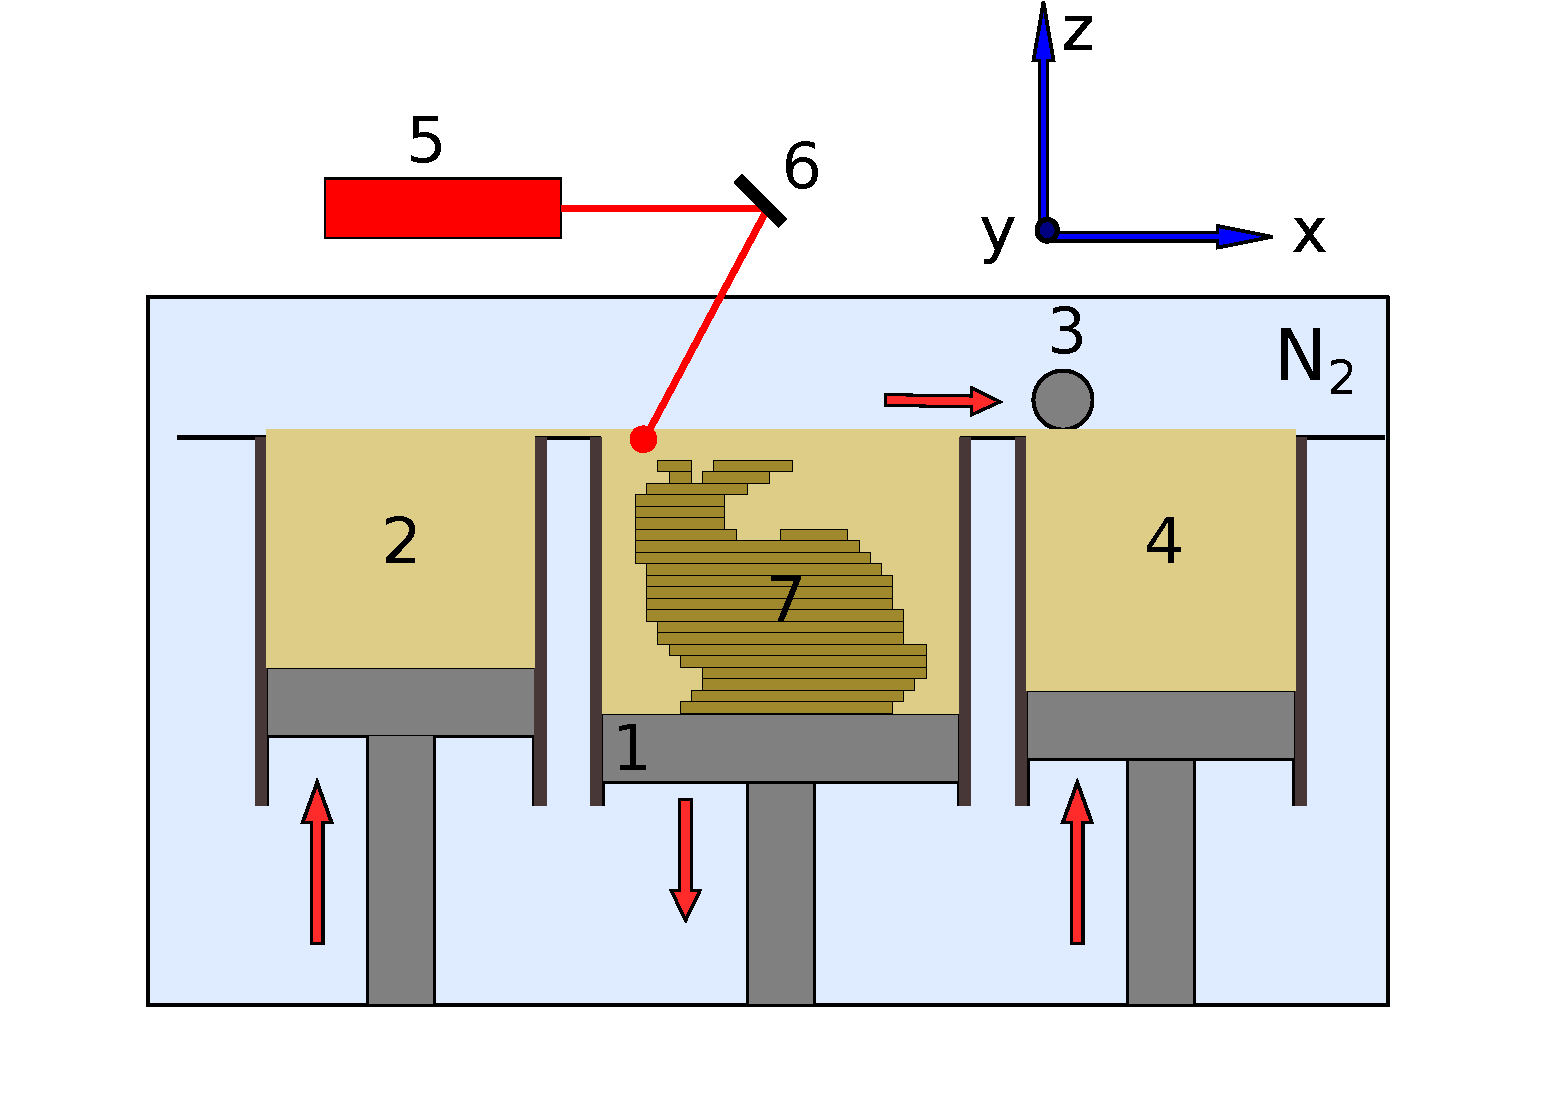
\includegraphics[width=\linewidth]{fig/sls-2d.pdf}
    \caption{Схематическое изображение работы СЛС-принтера.}
    \label{fig:printer}
\end{figure}


В процессе СЛС лазер послойно сканирует подложку с порошком и спекает частицы порошка, таким образом формируя заданную объемную структуру, как продемонстрированно на рис. \ref{fig:printer}. 







Порошок подается на сборочную платформу(1) из контейнера (2) и распределяется по ней тонким слоем с помощью ролика (3), двигающегося по оси $x$. Типичная толщина слоя составляет от 50 до 200 мкм. Остатки порошка собираются в контейнер (4).

CO2-лазер(-), снабженный оптикой(-), сканирует слой по заданным координатам

После сканирования каждого слоя, платформа сдвигается вниз по оси $z$ на глубину, равную толщине слоя. В процессе печати, так называемый колодец построения (5) "растет" снизу вверх. В объемном соотношении, он обычно состоит примерно на 90\% из неспеченного порошка, а изделие занимается только около 10\%. 

Как правило, перед спеканием порошок дополнительно прогревается.

В этой фазе, неспеченный порошок и расплавленные части остаются в квази-изотермических условиях внутри одного слоя.
Это температурное окно должно быть ниже, чем температура плавления, и выже чем температура рекристаллизации, для предотвращения коробления материала в процессе печати.
Для снижения окисления, камера purged азотом (остаточный кислород 2 \%). По завершению печати, part cake сначала охлаждается в атмосфере азота в течение примерно 10 ч, а затем охлаждается снаружи, пока температура не будет ниже температуры стеклования.

Затем, изделие отделяется от неспеченного порошка. В целом, при высоте изделия до 60 см, характерной толщиной слоя 100 мкм и временем сплавления на слой от 10 до 40 с, процес производства может занимать многие часы и дни, в результате старение материала. В связи с этим актуален синтез термостабильных материалов, как с точки зрения свойств конечного изделия, так и с точки зрения остаточного порошка, который затем желательно должен быть пригодным для повторной печати.



\paragraph{Особенности}
Помимо общих особенностей, характерных для технологий аддитивного производства, таких как..., селективное лазерное спекание также имеет свои преимущества.
\begin{itemize}
    \item хорошие характеристики изделий, сходные с традиционным производством.
    \item остатки порошка можно использовать повторно
    \item Напечатанные части остаются в неиспользованном порошке, поэтому, в отличие от других методом 3D-печати, не требуют специальных опорных конструкций.
    \item теоретически, обработке методом СЛС может успешно подвергаться любоее вещество, которое можно перевести в порошкообразное состояние и спечь при повышенной температуре\cite{vaganov}.
\end{itemize}



\subsection{Сращивание частиц порошка}

Высокая интенсивнсть лазерного излучения позволяет быстро нагревать небольшие участки материала, создавая большие градиенты температур \cite{sls-sim2016}.

Консолидация трехмерных изделий под воздействием лазерного излучения на полимерный материал, расположенный на "сборочной платформе" как правило называют селективным лазерным спеканием (СЛС, SLS) или селективым лазерным плавлением (SLM). Различие между СЛС и СЛП грубое, неопределенное и не охватывает все процессы, происходящие с порошком полимера под действием лазера.
Классификация схематически показана на рис.\ref{fig:binding}

It mainly deals with wax, ceramics [47–50], metals
[49,51–57] and polymers [58–63]. Major polymers used by SLS
include nylon, i.e. polyamide (PA) [60,61,63–68], (semi-) crystalline
thermoplastics: polyethylene [69–71] (PE), PEEK [72], and
PCL [73,74]. SLS can be categorized in solid state sintering (SSS),
liquid phase sintering-partial melting, full melting, and chemically
induced binding. SSS is a thermal process that occurs at temperatures
between TMelt/2 and TMelt, where TMelt is the melting temperature.
In liquid phase sintering-partial melting, usually the binder
material becomes liquefied, while structural material remains
solid. The full melting technique melts the powder entirely and
exhibits properties comparable to those of bulk material [75]. It
can be applied to a wide variety of materials, however, the long
process time and preheating of powders is necessary. Table 1 lists
the range of materials and their associated binding mechanism in
SLS.
CNT was added in Polyamide\cite{comp-review}


\begin{figure}[h]
    \centering
    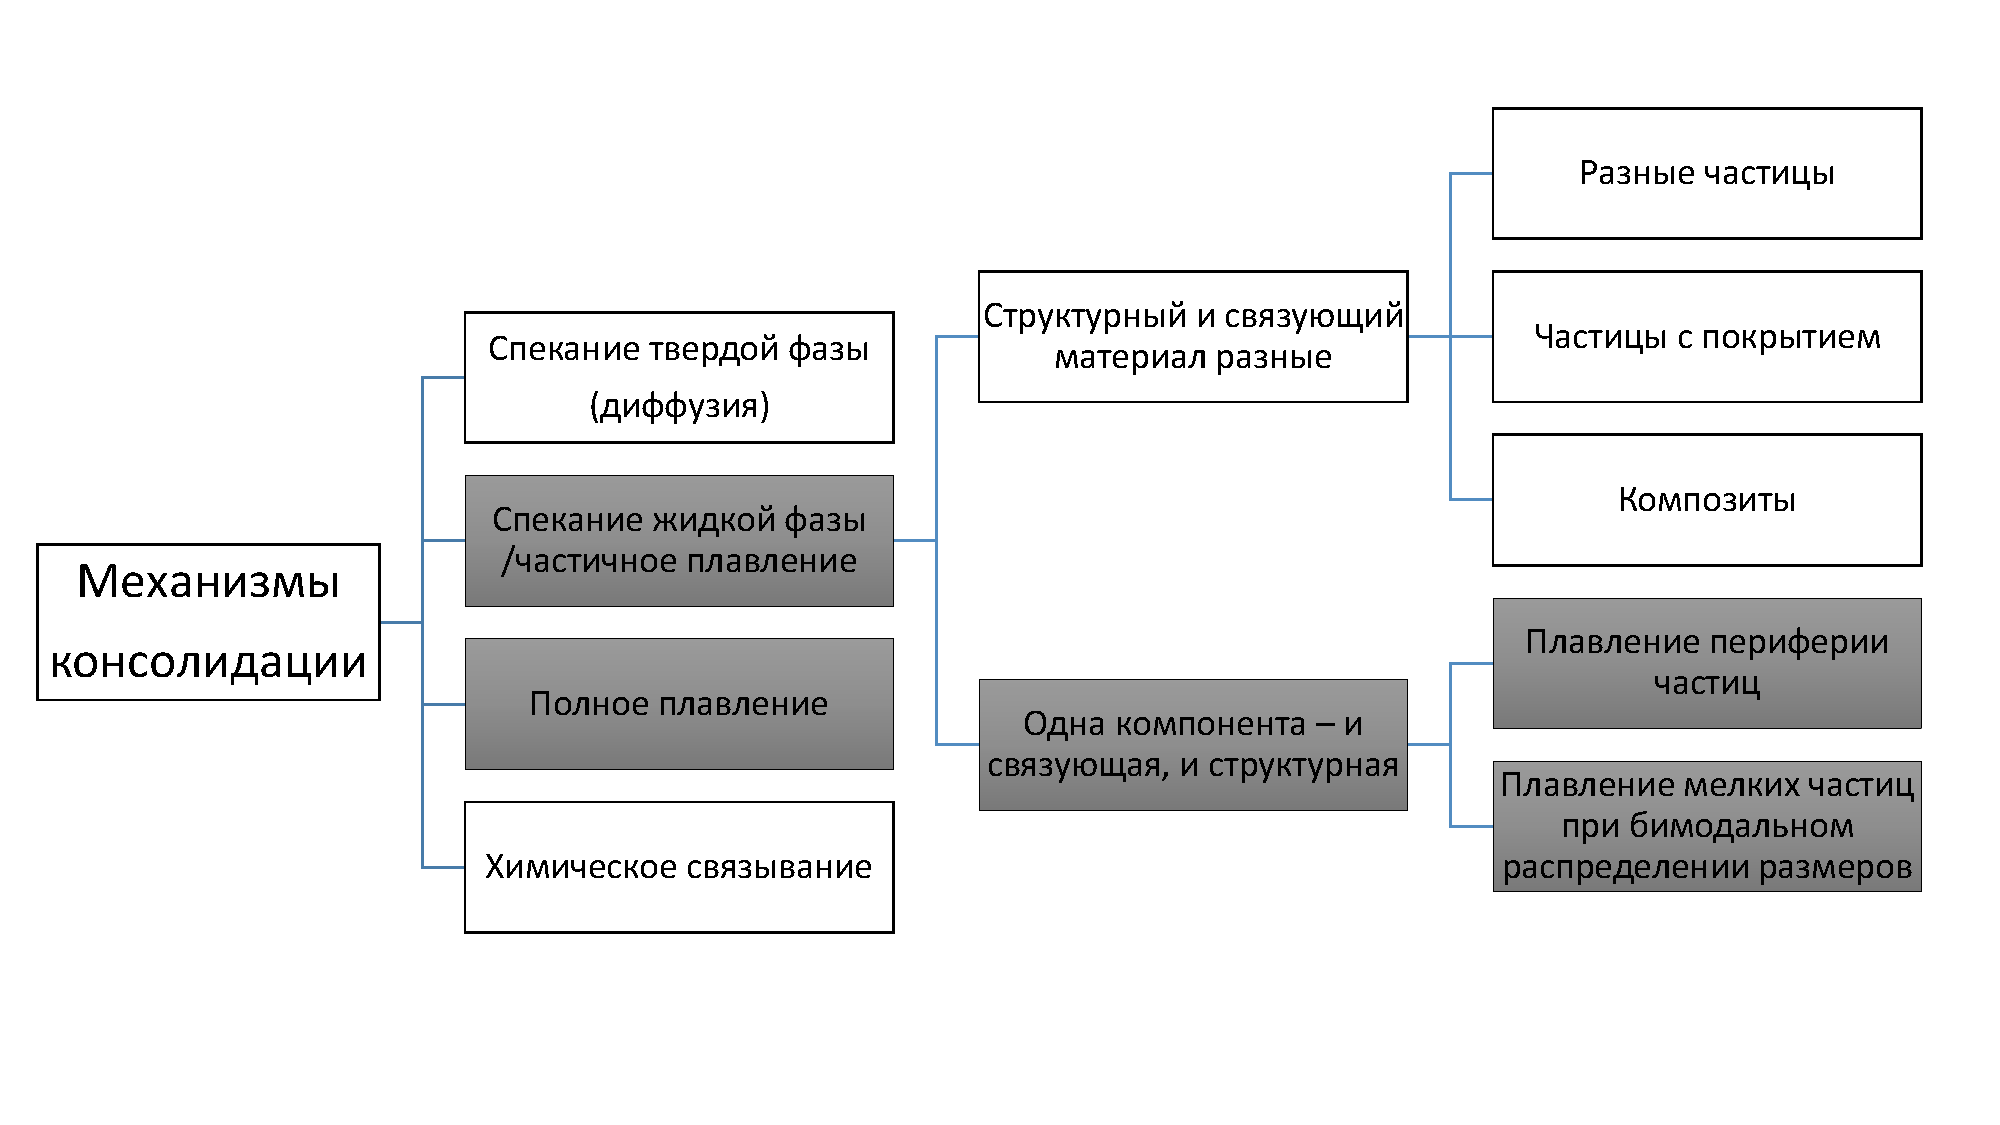
\includegraphics[width = \linewidth]{fig/mecha.pdf}
    \caption{Механизмы консолидации порошка}
    \label{fig:binding}
\end{figure}

\section{Требования к материалам для СЛС}

\subsection{Оценка эксплуатационных свойств}
Конечные характеристики изделия, полученного по технологии СЛС, во многом зависят от от свойств начального порошка  и параметров спекания (мощность лазера, скорость сканирования, диаметр пятна излучения лазера ).

Процесс производства выдвигает определенные требования к свойствам полимерных материалов, главным образом широкий диапазон рабочих температур large process window(?), низкая вязкость расплава, хорошая сыпучесть и высокий насыпной вес.
%Из-за этих ограничений, большинство применений СЛС сейчас основано на использовании полиамида 12.
Рассмотрим основные критерии оценки экспуатационных свойств полимерных материалов,\cite{termopols}.



Теплостойкость - формоустойчивость при нагревании
Гибкость цепей

Built parts are embedded in residual unmolten powder, the so-called part cake, which undergoes
thermal ageing effects due to the exposure to high temperatures for long times during the manufacturing process. Hence, the
recyclability of the unmolten powder is limited. \cite{ageing}


\subsection{Морфология частиц порошка}
Морфология частиц определяет пространственное расположение частиц порошка (stacking degree) относительно друг друга. Сферические (с гладкой поверхностью) частицы имеют высокую плотность упаковки. Они обеспечивают  сыпучесть in systems of applying the material with minimal resistance. В добавок, сферические частицы хорошо связываются в процессе спекания.Показано, что 
during the transition from powder particles with predominantly spherical morphology to particles of irregular shape of the same material, the elastic modulus decreases by almost 40 \%. 
(найти ссылку ,потом перевести).
Таким образом, сферический частицы с хорошей сыпучестью и высокой плотностью упаковки представляют идеальные характеристики стартового пороша для испольщования в СЛС.\\
В то же время использование частиц неправильной формы с большой вариацией в размерах ведет к созданию продуктов с более высокими механическими характеристиками в сравнении с использованием mainle сферических частиц с узким распределением размеров.

\subsection{Кристалличность}

\subsection{Полиэфиримиды ряда R-BAPB }
		
	\begin{figure}[h]
	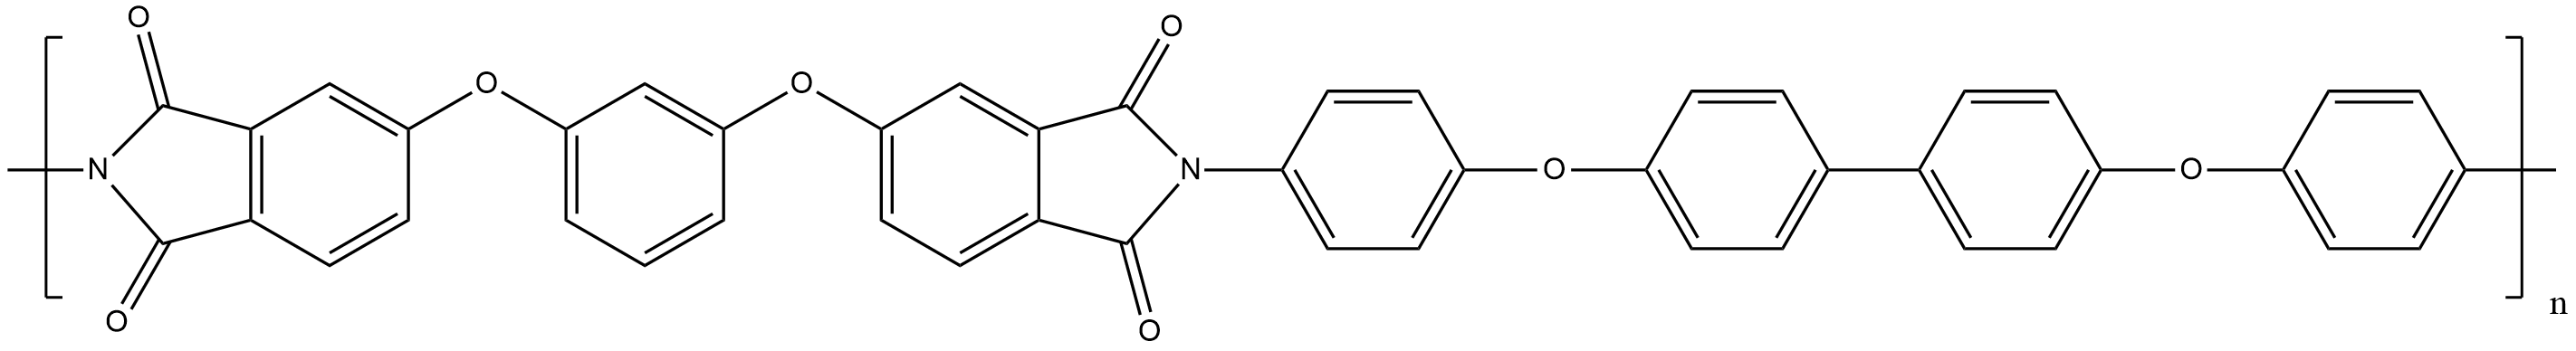
\includegraphics[width=\textwidth]{fig/formula.png}
	\caption{Структура полимера Р-ОДФО \cite{pi-formula}}
	\label{fig:formula}
	\end{figure}

Исследуемый в данной работе полимерный материал 


Что это\\
Особенности\\
Намеренные ранее характеристики\\
Использование в промышленности\\
Композиты\\
Короче, они збс и подходят для СЛС\\
Что нужно выяснить.\\

\section{Кристаллическая структура полимеров}

Что ее характеризует
Поскольку кристаллические области в этих полимерах формируются из длинных цепей, их кристаллизация сложна и сильно чувствительа к маленьким изменениям в полимерной (compostion), добавкам, температуре и механическим воздействиям.\\
Не все полимеры кристаллизуются, а те, что кристаллизуются, редко делают это полностью: только небольшая часть crystallizable цепей incorporated into crystalline domains, а остальные segregate into amorphous domains. Степеь кристалличности и характеристики кристаллических domains являются самыми важными морфологическими характеристиками, которые определяют физические свойства такие как плотность, mechanical strength, processability, permeability and degradability частичнокристаллического полимера.\\
Степень кристалличности типичного полимера варьируется в пределах от 10 до 80 \%. Сравните с металлами, которые, за исключением металлических стекол, почти всегда полностью кристалличны, и ceramics, которые или полностью кристалличны, или аморфны.\\ \cite{cryst3} или \cite{cryst1}






Кристаллическая структура полимеров менее идеальна чем кристаллы соединений с меньшей молекулярной массой. Как правило полимерные материалы находятся в метастабильном состоянии, то есть являются частично кристаллическими и частично аморфными. Большинсво полимеров частичнокристалличны по структуре, кристаллические структуры часто формируются при охлаждении расплава, что контролирует механические и физические свойства частичнокристаллических полимеров. Ввиду высокой вязкости полимерных расплавов, полимеры кристаллизуются очень медленно при температурах ниже температуры плавления ($T_m$), даже при высоком переохлаждении (high supercooling)
\\
Кристаллическая структура и степень кристалличости зависят от молекулярной структуры полимера, условий (growth
conditions), присутствия инородых частиц в решетке, температуры кристаллизации, скорости охлаждения и т.д.\\
Они могут быть оценены из рентгеновской дифракции, измерений плотности, термического аналища и т.д.

\subsection{Кристаллиты}
Морфологии полимерных кристаллов можно условно поделить на ламеллярные и фибриллярные кристаллы. В процессе ламеллярной кристаллизации, направление роста перпендикулярно направлению цепи, возникает складываение цепочки.Во время фибриллярной кристаллизации, наплавление роста кристалла совпадает с направление цепи, и в решетке кристалла возникают highly extended chain conformations. Такие материалы имеют высокие механические свойства. Кристаллизация существенно меняет физические и механические свойства полимерных систем. \\

Studying the crystallization
behavior, though complicated, is necessary mainly in relation to the physical and
mechanical properties of polymers. If crystallization would be absent in polymer
systems, then the whole mechanical performance of polymers depends on the glass
transition temperature (Tg). If glass transition is the only determining factor for the
properties of the polymers, then polymers such as polypropylene (PP) and PE
would have been rubbers at ambient temperature. However, in these polymers,
due to crystallization, the stiffness is retained at acceptable and controllable values
up to the melting temperature (Tm).\\
Multiphase polymer systems commonly consist of polymer blends, composites,
nanocomposites, interpenetrating polymer networks, block copolymers, and polymer
gels. Crystallization in multicomponent polymer-based systems represents the main
physical characteristic that allows for control of the material properties.\\
The presence of nanoparticles
can also limit themotion ofmolecular chains, resulting in suppression of the crystalline
perfection and crystallinity of polymer crystals.\\
Crystallization is a first-order transition and a thermal process in polymers. The
polymer chains are aligned and folded together to form an ordered chain region,
which is called lamellae. The lamellae are composed of spherical aggregates called
spherulites. The crystallization process changes the density, symmetry, and phase
transition and thus controls the properties of the end products. Crystallization
commonly proceeds by nucleation of a fiberlike structure followed by lamellar
structure formation. The spherulites grow away from a nucleation site.\\
Nowadays polymer composites are commonly used in aerospace, sport goods, automobiles,
industrial equipment, etc. Polymer composites are polymer-based matrix
with some form of materials embedded in the matrix, as reinforcements.\\
Polymer composites are classified on the basis of the size of filler particles into
microcomposites and nanocomposites.\\
(Это в планы на будущее)
Many experimental techniques can be used to study the crystallization
kinetics of nanocomposites. The most common techniques used to study the
crystallization kinetics in the nanocomposites are DSC, optical microscopy, and
WAXD.\\
The crystallization
kinetics of polymer composites and nanocomposites gained great interest due to the
fact that fillers act as an effective nucleating agent in the polymer matrix. With the
advancement of nanotechnology, the focus is now shifting toward understanding
the crystallization properties of materials in nanodimensions and thereby tune the
properties for diversified tailored application.\\

Это все из \cite{cryst1}

	\begin{wrapfigure}{r}{0.5\textwidth} 
\vspace{-20pt}


  \begin{center}
    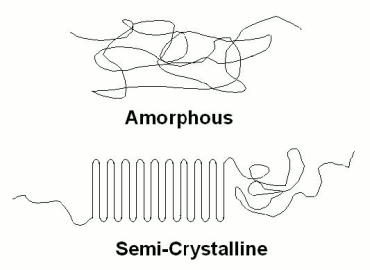
\includegraphics[width=0.4\textwidth]{fig/crystal-1.png}
    \caption{Как цепочки складываются в ламели}
    \label{fig:crystal-1}
  \end{center}
  \vspace{-20pt}
  \vspace{1pt}
\end{wrapfigure}



\begin{figure}[h]
    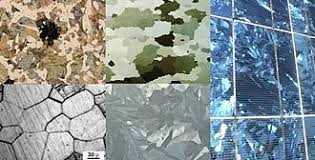
\includegraphics[width=\textwidth]{fig/crystallites.jpg}
    \caption{Типы кристаллитов}
    \label{fig:crystallites}
\end{figure}



\subsection{Частичная кристалличность}

Свойства частичнокристаллических полимеров можно понять, по большей части,
используя простую двухфазную модель, которая предполагает, что две фазы, кристаллическая и аморфная, легко различимы. Если интенсивный параметр  $\phi$ (например, удельный объем) кристаллической и аморфной фазы , $\phi_c$ и $\phi_c$, соответственно, может быть измерен, и мы предполагаем, что вклады двух фаз являются аддитивными, тогда
\[ 
\phi = \phi_c x + \phi_a(1-x),
\]
где $x$  -- доля кристаллической фазы, чаще всего массовая, хотя это в некоторой степени зависит от метода измерения \cite{cryst3}.

Простейшими организованными структурами, образуемыми полимерными цепями, являются кристаллиты, или ламели. Последние делее собираются в фибрилы или сферолиты. Возникновение сферолитов и фибрилл может
используется для определения, является ли полимер кристаллическим или нет, и для измерения локальной кристалличности.

Крупные образования, такие как сферолиты, можно наблюдать с помощью оптической микросопии, в то время как для обнаружения более мелких структур требуются другие методы -- например, электронная микроскопия, атомно-силовая микроскопия и т.д.

	\begin{wrapfigure}{r}{0.5\textwidth} 
\vspace{-20pt}
  \begin{center}
    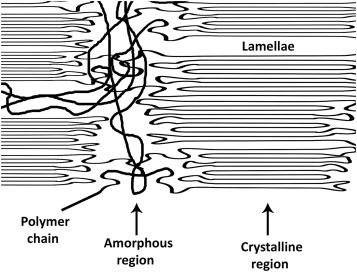
\includegraphics[width=0.4\textwidth]{fig/crystal-2.jpg}
    \caption{К определению кристалличности полимеров}
    \label{fig:crystal-2}
  \end{center}
  \vspace{-20pt}
  \vspace{1pt}
\end{wrapfigure}	

The two-phase model implied in Eq. (3.1) is only an approximation because
there can be a continuum of structures from large, defect-free single crystals to
the truly amorphous domains with liquid-like order. Because of the restrictions
imposed by long polymer chains, defects are invariably present in the crystal lattice,
and the polymer crystallites are small and disordered.\\
Conversely, the amorphous
domains possess some degree of positional and orientational correlations, and there
is experimental evidence for both rigid or ordered and soft or fluid amorphous phases\\
it may not always be possible to distinguish between the signatures
of the crystalline and amorphous phases. Nevertheless, a two-phase model with
an approximate crystalline phase and an amorphous phase, and sometimes an additional
ordered phase, mostly due to oriented amorphous domains, is often used.\\



\subsection{Влияние на макроскопические параметры}





	